With the representation of the symbol of high-order PDE operators given in Definition \ref{def:high_order_symbol}, we can derive the symbol of multigrid error propagation operators.

The total multigrid error propagation operator is given by
\begin{equation}
\mathbf{E}_{\text{TMG}} = {\color{burgundy}\mathbf{S}}_f \left( \mathbf{I} - {\color{burgundy}\mathbf{P}}_{\text{ctof}} {\color{burgundy}\mathbf{A}}_c^{-1} {\color{burgundy}\mathbf{R}}_{\text{ftoc}} {\color{burgundy}\mathbf{A}}_f \right) {\color{burgundy}\mathbf{S}}_f
\end{equation}
where ${\color{burgundy}\mathbf{S}}_f$ represents the smoother error propagation operator, while ${\color{burgundy}\mathbf{P}}_{\text{ctof}}$ and ${\color{burgundy}\mathbf{R}}_{\text{ftoc}}$ represent the grid prolongation and restriction operators between the coarse and fine grids, respectively.

\begin{definition}
The symbol of total multigrid error propegation operator for a finite element operator ${\color{burgundy}\mathbf{A}}$ is given by
\begin{equation}
\tilde{\mathbf{E}}_{\text{TMG}} \left( \mathbf{\theta} \right) = \tilde{{\color{burgundy}\mathbf{S}}}_f \left( \mathbf{\theta}, \omega \right) \left( \mathbf{I} - \tilde{{\color{burgundy}\mathbf{P}}}_{\text{ctof}} \left( \mathbf{\theta} \right) \left(\tilde{{\color{burgundy}\mathbf{A}}}_c \left( \mathbf{\theta} \right) \right)^{-1} \tilde{{\color{burgundy}\mathbf{R}}}_{\text{ftoc}} \left( \mathbf{\theta} \right) \tilde{{\color{burgundy}\mathbf{A}}}_f \left( \mathbf{\theta} \right) \right) \tilde{{\color{burgundy}\mathbf{S}}}_f \left( \mathbf{\theta}, \omega \right)
\end{equation}
where $\tilde{{\color{burgundy}\mathbf{S}}}_f$ represents the smoother error propagation symbol with any additional parameters $\omega$, while $\tilde{{\color{burgundy}\mathbf{P}}}_{\text{ctof}}$ and $\tilde{{\color{burgundy}\mathbf{R}}}_{\text{ftoc}}$ represent the grid prolongation and restriction symbols, respectively.
\label{def:multigrid_symbol}
\end{definition}

This error propagation operator can represent both h-multigrid and p-multigrid, depending upon the grid transfer operators and coarse grid representation chosen.

% -- P-Multigrid --------------------------------------------------------------
\subsection{P-Multigrid}

In p-multigrid, the different grids have the same number and size of finite elements but with different order basis functions.
The grid transfer operators can be represented elementwise and can thus be easily represented in the form of Equation \ref{eq:libceed_representation}.

The prolongation operator from the coarse to the fine grid interpolates low-order basis functions at the nodes for the high-order basis functions.
Figure \ref{fig:p_prolongation} shows the evaluation of second order basis function on the Gauss-Lobatto nodes for a fourth order basis.
This basis evaluation operation will be extended for LFA of h-multigrid and BDDC.

\begin{figure}[!ht]
  \centering
  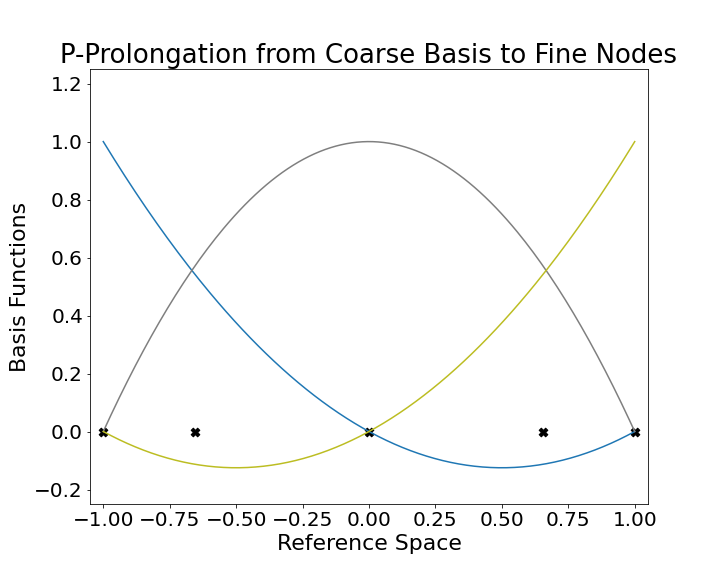
\includegraphics[width=0.48\textwidth]{../img/pProlongation}
  \caption{P-Prolongation from Coarse Basis to Fine Basis Points}
  \label{fig:p_prolongation}
\end{figure}

With this coarse to fine basis interpolation, the prolongation operator can be be represented by
\begin{equation}
\begin{tabular}{c}
${\color{burgundy}\mathbf{P}}_{\text{ctof}} = \mathbf{P}_f^T \mathbf{G}_f^T {\color{burgundy}\mathbf{P}}_e \mathbf{G}_c \mathbf{P}_c$\\
${\color{burgundy}\mathbf{P}}_e = {\color{blue(ncs)}\mathbf{I}} {\color{applegreen}\mathbf{D}}_{\text{scale}} {\color{blue(ncs)}\mathbf{B}}_{\text{ctof}}$
\end{tabular}
\end{equation}
where ${\color{blue(ncs)}\mathbf{B}}_{\text{ctof}}$ is an interpolation operator from the coarse grid basis to the fine grid basis, $\mathbf{P}_f$ and $\mathbf{G}_f$ are the fine grid element assembly operators, $\mathbf{P}_c$ and $\mathbf{G}_c$ are the coarse grid element assembly operators, and ${\color{applegreen}\mathbf{D}}_{\text{scale}}$ is a scaling operator to account for node multiplicity across element interfaces.
Restriction from the fine grid to the coarse grid is given by the transpose, ${\color{burgundy}\mathbf{R}}_{\text{ftoc}} = {\color{burgundy}\mathbf{P}}_{\text{ctof}}^T$.

It is useful to think of the p-prolongation operation as an interpolation operation between the coarse and fine grids, but in practice it can be easier to construct the prolongation basis ${\color{blue(ncs)}\mathbf{B}}_{\text{ctof}}$ from the coarse and fine grid interpolation operators, provided that both bases use the same quadrature space.
\begin{equation}
\begin{tabular}{c c}
${\color{blue(ncs)}\mathbf{B}}_f = \mathbf{Q} \mathbf{R},$ & ${\color{blue(ncs)}\mathbf{B}}_{\text{ctof}} = \mathbf{R}^{-1} \mathbf{Q}^T {\color{blue(ncs)}\mathbf{B}}_c$
\end{tabular}
\label{eq:p_prolong_basis}
\end{equation}
In Equation \ref{eq:p_prolong_basis}, we form the interpolation operation between the coarse grid from the coarse grid interpotation operator and the QR factorization of the fine grid interpolation operator.
Note that in the case of H1 Lagrange bases, this factorization will produce the same coarse to fine grid interpolation operator as evaluating the coarse grid basis functions at the fine grid nodes.

Following the derivation from Section \ref{sec:lfahighorder}, we can derive the symbols of ${\color{burgundy}\mathbf{P}}_{\text{ctof}}$ and ${\color{burgundy}\mathbf{R}}_{\text{ftoc}}$.

\begin{definition}
The symbol of the p-prolongation operator is given by
\begin{equation}
\tilde{{\color{burgundy}\mathbf{P}}}_{\text{ctof}} \left( \theta \right) = \mathbf{Q}_f^T \left( {\color{burgundy}\mathbf{P}}_e \odot \left[ e^{\imath \sum_d \left( \mathbf{x}_{i, f} - \mathbf{x}_{j, c} \right) \mathbf{\theta} / \mathbf{h}} \right] \right) \mathbf{Q}_c
\end{equation}
where $i \in \left[ 0, 1, \dots, \left( p_{\text{fine}} \right)^{\text{dim}} \right]$, $h$ is the length of the element, and $j \in \left[ 0, 1, \dots, \left( p_{\text{coarse}} \right)^{\text{dim}} \right]$.
The matrices $\mathbf{Q}_f$ and $\mathbf{Q}_c$ are the localization mappings for the fine and coarse grid, respectively, and the element p-prolongation operator is given by ${\color{burgundy}\mathbf{P}}_e = {\color{blue(ncs)}\mathbf{I}} {\color{applegreen}\mathbf{D}}_{\text{scale}} {\color{blue(ncs)}\mathbf{B}}_{\text{ctof}}$.
\label{def:p_prolongation_symbol}
\end{definition}

\begin{definition}
The symbol of p-restriction operator is given by the expression
\begin{equation}
\tilde{{\color{burgundy}\mathbf{R}}}_{\text{ftoc}} \left( \theta \right) = \mathbf{Q}_c^T \left( {\color{burgundy}\mathbf{R}}_e \odot \left[ e^{\imath \sum_d \left( \mathbf{x}_{i, c} - \mathbf{x}_{j, f} \right) \mathbf{\theta} / \mathbf{h}} \right] \right) \mathbf{Q}_f
\end{equation}
where $i \in \left[ 0, 1, \dots, \left( p_{\text{coarse}} \right)^{\text{dim}} \right]$, $h$ is the length of the element, and $j \in \left[ 0, 1, \dots, \left( p_{\text{fine}} \right)^{\text{dim}} \right]$.
The matrices $\mathbf{Q}_f$ and $\mathbf{Q}_c$ are the localization mappings for the fine and coarse grid, respectively, and the element p-restriction operator is given by ${\color{burgundy}\mathbf{R}}_e = {\color{burgundy}\mathbf{P}}_e^T = {\color{blue(ncs)}\mathbf{B}}_{\text{ctof}}^T {\color{applegreen}\mathbf{D}}_{\text{scale}} {\color{blue(ncs)}\mathbf{I}}$.
\label{def:p_restriction_symbol}
\end{definition}

\begin{figure}[!h]
  \centering
  \subfloat[Spectrum of P-Multigrid for $p_f = 4$, $p_c = 2$]{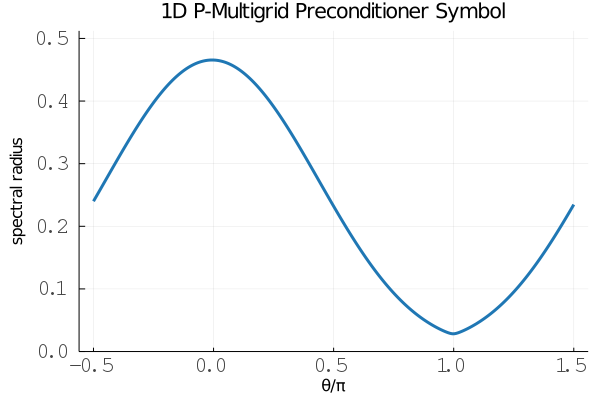
\includegraphics[width=0.48\textwidth]{../img/pmultigridSymbol1D}\label{fig:p_multigrid_spectrum_1d}}
  \hfill
  \subfloat[Spectrum of P-Multigrid for $p_f = 4$, $p_c = 2$]{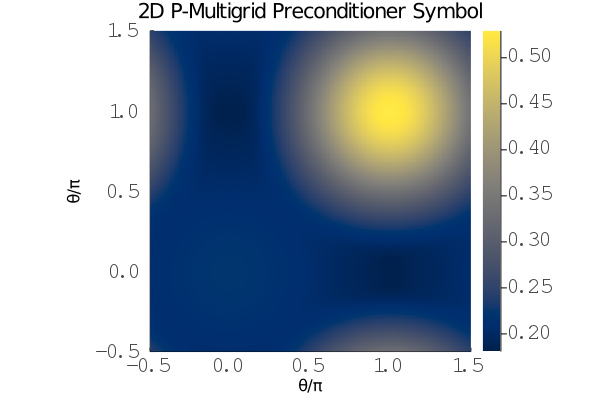
\includegraphics[width=0.48\textwidth]{../img/pmultigridSymbol2D}\label{fig:p_multigrid_spectrum_2d}}
  \caption{Spectrum of Spectrum of P-Multigrid Symbol for $p_f = 4$, $p_c = 2$}
\end{figure}

In Figures \ref{fig:p_multigrid_spectrum_1d} and \ref{fig:p_multigrid_spectrum_2d}, we see the spectral radius of the symbol of p-multigrid for the scalar diffusion operator with third-order Chebyshev smoothing on a fine grid with a fourth-order H1 Lagrange finite element basis and a coarse grid with a second-order H1 Lagrange finite element basis on the Gauss-Lobatto points in one and two dimensions.
Various preconditioning techniques will reduce this spectral radius, with different effectiveness in different frequency ranges.

% -- H-Multigrid --------------------------------------------------------------
\subsection{H-Multigrid}

In h-multigrid, the different grids have the same polynomial order of finite elements but these elements are amalgamated into increasingly larger elements.
For LFA of h-multigrid, we introduce the concept of macro-element bases.
With macro-element bases, the grid transfer operators can be still represented elementwise and can thus be easily represented in the form of Equation \ref{eq:libceed_representation}.

A macro-element basis is formed by amalgamating two or more finite element bases.
Each micro-element has separate quadrature spaces, so the basis functions for each sub-element, or micro-element, are defined as zero on the portions of the domain not included in the given micro-element.
In effect, the basis interpolation and gradient operations for the macro-element provide a micro-element restriction and micro-element basis operation together.

\begin{figure}[!ht]
  \centering
  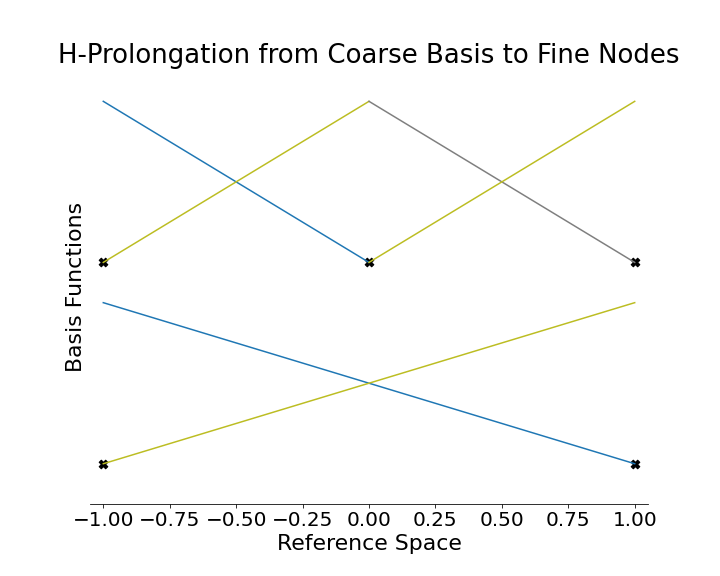
\includegraphics[width=0.48\textwidth]{../img/hProlongation}
  \caption{H-Prolongation from Coarse Basis to Fine Basis Points}
  \label{fig:h_prolongation}
\end{figure}

In Figure \ref{fig:h_prolongation}, we see an example of interpolation from a coarse grid basis to a fine grid macro-element basis.
The linear shape functions are evaluated at the nodes of the fine grid macro-element, which is a pair of linear micro-elements.
On the left linear micro-element, there are two basis functions which are zero over the domain of the right micro-element, and the reverse is also true.
The element level operator, ${\color{burgundy}\mathbf{A}}_e$, on the fine grid macro-element assembles the element level operator for each micro-element into the action of the PDE operator on the full macro-element.

With this macro-element structure, we can form the Fourier mode localization operator for the macro-element in the same fashion as the Fourier mode localization operator for high-order elements given in Equation \ref{eq:fouriermodelocalization1d}.
With macro-elements, there are $n * p$ columns in the localization operator for a one dimensional scalar PDE on a marco-element with $n$ micro-elements instead of $p$ columns for a one dimensional scalar PDE on a single high order element.
\begin{equation}
\mathbf{Q} =
\begin{bmatrix}
    I   \\
    e_0 \\
\end{bmatrix} =
\begin{bmatrix}
    1      && 0      && \cdots && 0      \\
    0      && 1      && \cdots && 0      \\
    \vdots && \vdots && \vdots && \vdots \\
    0      && 0      && \cdots && 1      \\
    1      && 0      && \cdots && 0      \\
\end{bmatrix}
\end{equation}

Following the derivation from Section \ref{sec:lfahighorder}, we can derive the symbols of ${\color{burgundy}\mathbf{P}}_{\text{ctof}}$ and ${\color{burgundy}\mathbf{R}}_{\text{ftoc}}$.

\begin{definition}
The symbol of the h-prolongation operator is given by
\begin{equation}
\tilde{{\color{burgundy}\mathbf{P}}}_{\text{ctof}} \left( \theta \right) = \mathbf{Q}_f^T \left( {\color{burgundy}\mathbf{P}}_e \odot \left[ e^{\imath \sum_d \left( \mathbf{x}_{i, f} - \mathbf{x}_{j, c} \right) \mathbf{\theta} / \mathbf{h}} \right] \right) \mathbf{Q}_c
\end{equation}
where $i \in \left[ 0, 1, \dots, \left( p * n \right)^d \right]$, $h$ is the length of the macro-element, $j \in \left[ 0, 1, \dots, p^d \right]$, $d$ is the dimension of the finite element bases, and $n$ is the number of micro-elements in each fine grid macro-element.
The matrices $\mathbf{Q}_f$ and $\mathbf{Q}_c$ are the localization mappings for the fine and coarse grid, respectively, and the macro-element h-prolongation operator is given by ${\color{burgundy}\mathbf{P}}_e = {\color{blue(ncs)}\mathbf{I}} {\color{applegreen}\mathbf{D}}_{\text{scale}} {\color{blue(ncs)}\mathbf{B}}_{\text{ctof}}$.
\label{def:h_prolongation_symbol}
\end{definition}

\begin{definition}
The symbol of h-restriction operator is given by the expression
\begin{equation}
\tilde{{\color{burgundy}\mathbf{R}}}_{\text{ftoc}} \left( \theta \right) = \mathbf{Q}_c^T \left( {\color{burgundy}\mathbf{R}}_e \odot \left[ e^{\imath \sum_d \left( \mathbf{x}_{i, c} - \mathbf{x}_{j, f} \right) \mathbf{\theta} / \mathbf{h}} \right] \right) \mathbf{Q}_f
\end{equation}
where $i \in \left[ 0, 1, \dots, p^d \right]$, $h$ is the length of the macro-element, $j \in \left[ 0, 1, \dots, \left( p * n \right)^d \right]$, $d$ is the dimension of the finite element bases, and $n$ is the number of micro-elements in each fine grid macro-element.
The matrices $\mathbf{Q}_f$ and $\mathbf{Q}_c$ are the localization mappings for the fine and coarse grid, respectively, and the macro-element h-restriction operator is given by ${\color{burgundy}\mathbf{R}}_e = {\color{burgundy}\mathbf{P}}_e^T = {\color{blue(ncs)}\mathbf{B}}_{\text{ctof}}^T {\color{applegreen}\mathbf{D}}_{\text{scale}} {\color{blue(ncs)}\mathbf{I}}$.
\label{def:h_restriction_symbol}
\end{definition}

\begin{figure}[!h]
  \centering
  \subfloat[Spectrum of H-Multigrid for $p = 1$]{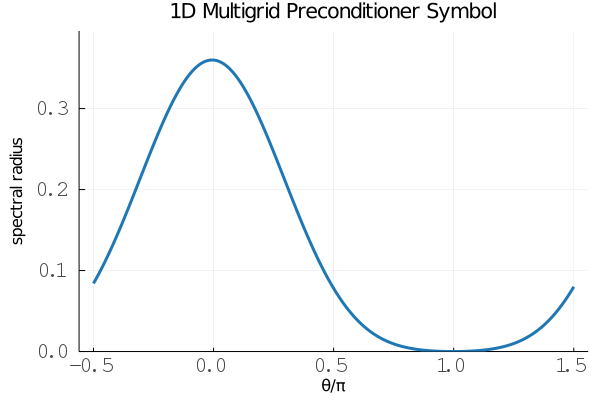
\includegraphics[width=0.48\textwidth]{../img/hmultigridSymbol1D}\label{fig:h_multigrid_spectrum_1d}}
  \hfill
  \subfloat[Spectrum of H-Multigrid for $p = 1$]{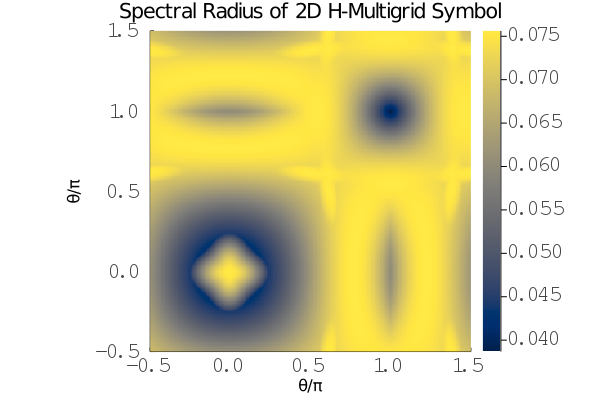
\includegraphics[width=0.48\textwidth]{../img/hmultigridSymbol2D}\label{fig:h_multigrid_spectrum_2d}}
  \caption{Spectrum of Spectrum of H-Multigrid Symbol for $p = 1$}
\end{figure}

In Figures \ref{fig:h_multigrid_spectrum_1d} and \ref{fig:h_multigrid_spectrum_2d}, we see the spectral radius of the symbol of h-multigrid for the scalar diffusion operator with third-order Chebyshev smoothing on a fine grid with a fourth-order H1 Lagrange finite element basis and a coarse grid with a second-order H1 Lagrange finite element basis on the Gauss-Lobatto points in one and two dimensions.
Various preconditioning techniques will reduce this spectral radius, with different effectiveness in different frequency ranges.
